% Section 3: method. Numbers: generated/numbers.tex.
\section{Estimation method}\label{sec:method}

\subsection{Observation model}\label{sec:obs}
Pass $i$ is a record of vertical axle-box acceleration over \NumRevs{} wheel revolutions, so its
length is fixed in space, $L = \NumRevs\cdot 2\pi r_0$, and its duration $T_i = L/V_i$ depends on the
pass speed $V_i$. The DFT coefficient $c_{ik}$ at bin $k$ belongs to the frequency $f_{ik} = k/T_i$
and to the same wavenumber $\gamma_k = 2\pi k/L$ on every pass. The analysis band is fixed in
frequency.

Rail roughness is a stationary Gaussian process with one-sided wavenumber spectrum
\begin{equation}
  G(\gamma) = G_\mathrm{ISO}(\gamma)\,g_{s(\gamma)},
\end{equation}
where $G_\mathrm{ISO}$ has the shape of the ISO~3095 limit spectrum~\citep{iso3095} and
$g_s$ is a free level in sub-band $s$, with $K$ sub-bands per one-third octave. The levels are
nuisance parameters: the method never measures roughness. The axle load of each pass, $W_i$, is a
nuisance with a Gaussian prior on $\log W_i$ centred on a weigh-in-motion reading with standard
deviation \WIMsigmaPct\%. The sensor noise is white with level $e_i$, estimated from an
out-of-band part of the same record. The globals $\bm\theta$ are the health parameters
$(k_{B0}, c_B)$, optionally with track parameters such as $k_f$ and $k_{H0}$.

Under this model the coefficients are approximately independent complex Gaussians with variance
\begin{equation}
  v_{ik} = |H(f_{ik};\bm\theta, W_i, V_i)|^2\, 2G(\gamma_k)\,\Delta\gamma + e_i,
  \label{eq:binvar}
\end{equation}
and the negative log-likelihood over $N$ passes is the multi-pass Whittle form~\citep{whittle1953}
\begin{equation}
  \ell(\bm\theta, \bm g, \bm W) = \sum_{i=1}^{N}\sum_k\left[\log v_{ik} + \frac{|c_{ik}|^2}{v_{ik}}\right]
  + \sum_{i=1}^{N}\frac{(\log W_i - \log\hat W_i)^2}{2\sigma_W^2}.
  \label{eq:whittle}
\end{equation}
The same structure, with the modal-force spectrum per band as the nuisance, underlies Bayesian
FFT operational modal analysis~\citep{au2011}.

\paragraph{Why speed diversity identifies the support.} Roughness is fixed in wavenumber, while the
resonance of the axlebox on its support is fixed in frequency. A pass at speed $V_i$ maps
wavenumber $\gamma$ to frequency $V_i\gamma/2\pi$, so passes at different speeds see the same
roughness sub-band through different parts of $|H|^2$. With a single speed, a change of $|H|^2$ and
a change of roughness level are indistinguishable sub-band by sub-band; with a spread of speeds
they separate. Figure~\ref{fig:crb-speed} shows the Cram\'er--Rao bound of $k_{B0}$ falling with
the speed spread for several sub-band resolutions $K$.

\begin{figure}[tbp]\centering
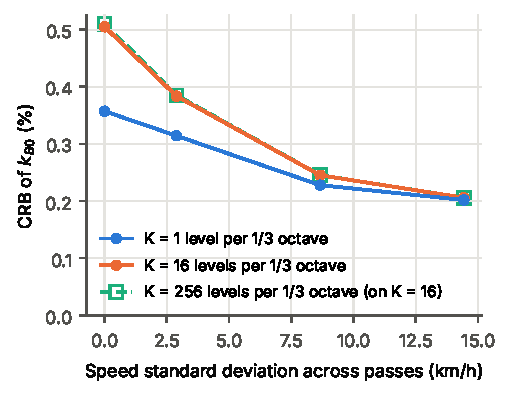
\includegraphics[width=0.55\textwidth]{fig2_crb_vs_speed_spread}
\caption{Effect of speed spread on identifiability. Cram\'er--Rao bound of $k_{B0}$ against the speed spread across passes, for $K$ roughness
levels per one-third octave ($N=50$, 40~dB, payload spread). Data:
\texttt{results/p1/bound\_speed\_subband.json}.}
\label{fig:crb-speed}
\end{figure}

\subsection{Debiased likelihood for multi-wheel cross terms}\label{sec:debias}
Equation~\eqref{eq:binvar} samples $|H|^2G$ at the bin. The expected periodogram of a finite
record is instead the spectrum convolved with the Fej\'er kernel $T\,\mathrm{sinc}^2((f-f_k)T)$.
The two agree when the spectrum is smooth on the scale of one bin, as for a single wheelset. They
do not agree once the multi-wheel phase factors in~\eqref{eq:H} put ripples of period $V/(d_k-d_j)$
close to the bin width. Following Sykulski et al.~\citep{sykulski2019}, we keep the Whittle form but
replace $v_{ik}$ by the exact expected periodogram,
\begin{equation}
  v_{ik} = \sum_m \frac{\mathrm{sinc}^2\!\big((f_m - f_{ik})T_i\big)}{M}\,
           |H(f_m)|^2\,2G(\gamma_m)\,\Delta\gamma + e_i,
  \label{eq:debiased}
\end{equation}
with the sum over a grid $M=\KernelFine$ times finer than the bins, truncated at $\pm\KernelHalfWidth$ bins
(a narrower truncation at $\pm30$ bins leaves a measurable bias; Section~\ref{sec:res-bias}). On the
simulated 12-wheel setup of~\citep{carrigan2023}, the bin-sampled model differs from the mean of
\DebiasRecords{} periodograms by an rms log-ratio of \DebiasBin{}; the debiased model differs by
\DebiasDeb{}, against \DebiasNoise{} expected from sampling alone (Fig.~\ref{fig:debias}).

\begin{figure}[tbp]\centering
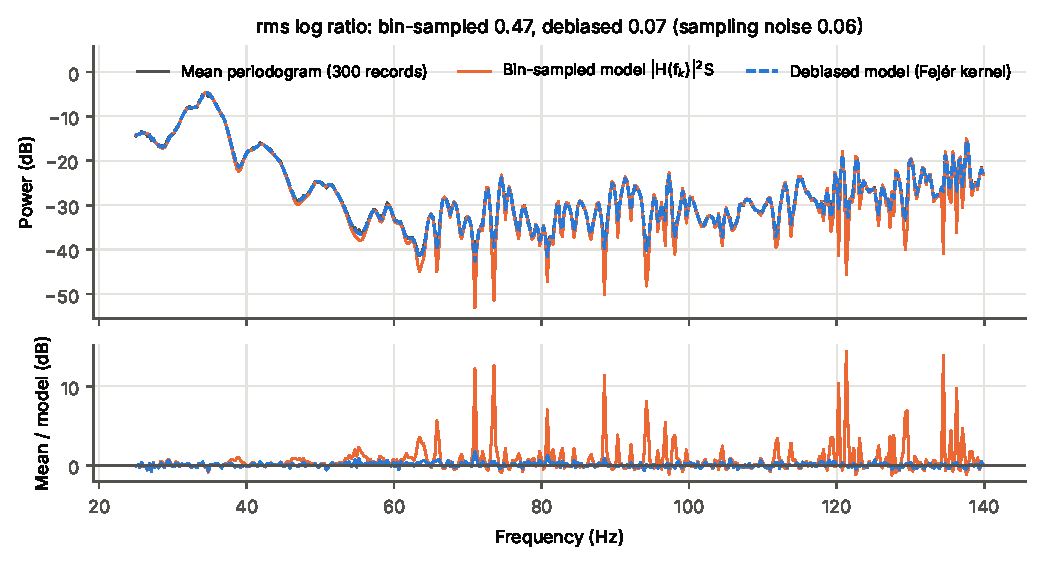
\includegraphics[width=\textwidth]{fig3_debiased_periodogram}
\caption{Check of the debiased likelihood. Mean periodogram of \DebiasRecords{} records against the bin-sampled and the debiased
(Fej\'er-convolved) models (top) and their ratio (bottom). Data:
\texttt{results/p2/debias\_check.json}.}
\label{fig:debias}
\end{figure}

\subsection{Profiling and optimisation}\label{sec:profile}
For given globals $\bm\theta$, the nuisances $(\log\bm g, \log\bm W)$ are profiled out by Fisher
scoring, warm-started from the previous evaluation. The globals are then found by Nelder--Mead on
the profile likelihood. With the debiased variance~\eqref{eq:debiased} the kernel mixes
neighbouring roughness sub-bands. The default scoring step attributes each bin's variance to its
own sub-band; the exact step uses the full derivative $\partial v_{ik}/\partial\log g_s$ over all
sub-bands and the corresponding Fisher matrix, so that its fixed point is the exact profile maximum.
Section~\ref{sec:res-bias} compares the two.

The transfer functions are computed directly from the finite-element and rail models (no
surrogate): a table of the coupled components $G_k(f;\bm\theta,W)$ over payload nodes, built from an
exact modal decomposition of the wheelset for each trial $\bm\theta$, is interpolated in $\log W$
and frequency.

\subsection{Uncertainty}\label{sec:uncertainty}
Wald intervals use the observed information of the profile likelihood (numerical Hessian).
Profile-likelihood intervals use the $\chi^2_1$ cut, re-optimising the other globals and all
nuisances. The Cram\'er--Rao bound (CRB) is the inverse expected Fisher information with every
nuisance free and the weigh-in-motion prior included. When records repeat over the same section,
the independence assumed in~\eqref{eq:whittle} fails across passes; the variance is then taken
from a sandwich estimator clustered on DFT bin (the same wavenumber on every pass).
Where the Wald intervals under-cover in simulation (Section~\ref{sec:res-headline}), they are
simulation-calibrated for the design: the mean bias of $\log\hat k_{B0}$ found by simulation is
subtracted and the standard error is multiplied by the simulated ratio of RMSE to standard error,
checked on held-out simulation seeds.

\subsection{Relative change and detection}\label{sec:relative}
The monitoring output is the change of support stiffness between a baseline period and a later
period of the same vehicle and sensor, each with $N$ passes in the same payload band. Two bands are used:
empty (axle load 5.5--7~t) and laden (20--22.5~t); in each, the estimator uses the band's primary
stiffness and damping (Table~\ref{tab:table1_parameters}), and the weigh-in-motion payload assigns each
pass to its band. Pooling passes over the whole payload range requires a payload-dependent model of the
primary suspension (Section~\ref{sec:res-primary}). The change is

\begin{equation}
  D = \log\hat k_{B0}^{\,\mathrm{later}} - \log\hat k_{B0}^{\,\mathrm{base}},
\end{equation}
reported as $\Delta k_{B0}/k_{B0} = \exp(D)-1$. A misspecified model parameter biases $\log\hat k_{B0}$
in both periods; to first order the common part cancels, and the remainder scales with the change
itself. We therefore use the interval
\begin{equation}
  D \pm 1.645\sqrt{\mathrm{se}_\mathrm{base}^2 + \mathrm{se}_\mathrm{later}^2 + (\kappa D)^2},
  \label{eq:interval}
\end{equation}
where $\kappa$ is the model-form gain uncertainty: the root sum of squares, over the uncertain model
parameters, of the gain $\partial(\hat D/D)/\partial\log(\text{parameter})$ times that parameter's
$1\sigma$ log range. Foundation stiffness can drift between periods (seasonal pad stiffness), so the
default fit re-estimates $k_f$ and $k_{H0}$ in each period together with $(k_{B0}, c_B)$.

A loss is declared when $D < -1.645\,s_0$, where $s_0$ is the standard deviation of $D$ with no
change (5\% false-alarm rate, one-sided). The minimum detectable change (MDC) is the true decrease
detected with probability 0.9, $\mathrm{MDC} = (1.645 + 1.282)\,s_0$ without bias; with a bias in
$D$ it is found by interpolating the bias against the true change.

\subsection{Model-form bias}\label{sec:pseudotrue}
The large-sample bias under a misspecified model is the pseudo-true parameter: the minimiser of the
expected value of~\eqref{eq:whittle} when the periodograms are replaced by their expectations under
the true model. It is computed by the same profiled fit with $|c_{ik}|^2$ replaced by the true
$v_{ik}$, and was checked against full Monte Carlo fits. A first-order (score) approximation was
found to fail for large parameter errors and is not used.

\subsection{Implementation and use of AI}\label{sec:implementation}
The simulation and estimation code was developed with the assistance of an AI coding tool, Claude Code
(developer: Anthropic; model: Claude Opus 5.5). It was used to write the code (the finite-element and
rail models, the simulation and estimation scripts, and the scripts that generate tables, figures and
the numbers quoted in the text) and to assist the literature search. All code was reviewed, tested and
verified by the authors: unit tests cover the finite-element and rail models, the model is verified
against closed-form solutions (Table~\ref{tab:table2_verification}), and every result in this paper is
regenerated by script from stored, version-controlled result files.
